%%% Preamble
\documentclass[paper=letter, fontsize=10pt]{scrartcl}	% Article class of KOMA-script with 11pt font and a4 format

\usepackage[english]{babel}							
\usepackage[margin=1in]{geometry}
%TIKZ
\usepackage{tikz}
\usetikzlibrary{shapes,arrows}
\usepackage{pgfplots} %ADDED FOR Figure

%%PACKAGES FOR CODE DISPLAY
\usepackage{floatrow}
\usepackage{minted}    
\floatsetup[listing]{style=Plaintop}  

% load package with ``framed'' and ``numbered'' option.
\usepackage[framed,numbered,autolinebreaks,useliterate]{mcode}

% English language/hyphenation
\usepackage[protrusion=true,expansion=true]{microtype}  % Better typography
\usepackage{amsmath,amsfonts,amsthm}			% Math packages
\usepackage[hang, small,labelfont=bf,up,textfont=it,up]{caption}	% Custom captions under/above floats
\usepackage{epstopdf}				
\usepackage{subfig}								% Subfigures
\usepackage{booktabs}							% Nicer tables

%%% Advanced verbatim environment
\usepackage{verbatim}
\usepackage{fancyvrb}
\DefineShortVerb{\|}		% delimiter to display inline verbatim text


%%% Custom sectioning (sectsty package)
\usepackage{sectsty}			% Custom sectioning (see below)
\allsectionsfont{%			% Change font of al section commands
	\usefont{OT1}{bch}{b}{n}%% bch-b-n: CharterBT-Bold font
%	\hspace{15pt}%			% Uncomment for indentation
	}

\sectionfont{%		% Change font of \section command
	\usefont{OT1}{bch}{b}{n}%	% bch-b-n: CharterBT-Bold font
	\sectionrule{0pt}{0pt}{-5pt}{0.8pt}% % Horizontal rule below section
	}


%%% Custom headers/footers (fancyhdr package)
\usepackage{fancyhdr}
\pagestyle{fancyplain}
\fancyhead{}						% No page header
\fancyfoot[C]{\thepage}		% Pagenumbering at center of footer
\fancyfoot[R]{\small \texttt{Midterm Project Update}}	% You can remove/edit this line 
\renewcommand{\headrulewidth}{0pt}	% Remove header underlines
\renewcommand{\footrulewidth}{0pt}	% Remove footer underlines
\setlength{\headheight}{13.6pt}

%%% Equation and float numbering
\numberwithin{equation}{section}															% Equationnumbering: section.eq#
\numberwithin{figure}{section}																% Figurenumbering: section.fig#
\numberwithin{table}{section}																% Tablenumbering: section.tab#

%%% Title	
\title{ \vspace{-.25in} 	\usefont{OT1}{bch}{b}{n}
		\huge \strut EECS567 Midterm Report \strut \\
		\Large \bfseries \strut Resolved Motion Rate Control Algorithm: \\* Simulation and Implementation  \strut
}
\author{ 									\usefont{OT1}{bch}{m}{n}
        Kris Schilling, Ran Lin, and Yang Xu\\		\usefont{OT1}{bch}{m}{n}
        University of Michigan\\	\usefont{OT1}{bch}{m}{n}
        Mechanical Engineering Department\\
}
\date{}

%%% Begin document
\begin{document}
\maketitle
\section{Introduction}
This paper is intended to give the details of our EECS567 semester project.

\subsection{Motivation}
Many industrial applications require the end-effector of a robot to move along a desired path at a set velocity. The ability to easily adapt a robotic manipulator for various tasks gives the manufacture a cost benefit of purchasing multiple manipulators and allows for Lean Manufacturing. As opposed to calculating the inverse kinematic equation geometrically, we will review the Resolved Motion Rate Control (RMRC) discussed in \cite{whitney1969resolved}. The benefits the method can provide apply to open loop and closed loop control. For example, a human using a joystick to control a robot expects control in the direction specified at a speed proportional to the input. In this project, our team wants to review the RMRC method, overview the benefits and limitations, and get experience implementing the algorithm on physical hardware.

\begin{figure}[h!]
  \centering
    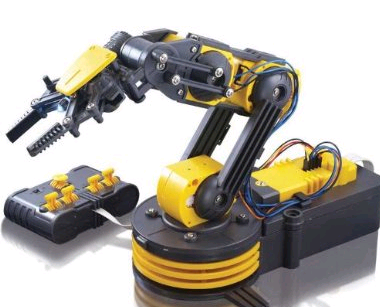
\includegraphics[width=0.3\textwidth]{./Images/OWI}
    \caption{OWI ARM}
    \label{fig:OWI}
\end{figure}

\subsection{Objective}
The object of the project will be to implement a Rate Motion Control algorithm using a low-cost commercial off the shelf (COTS) robotic manipulator. The mathematics derivations of the Resolved Motion Rate Control will first be derived. Following this, we will define the DH parameters for the OWI robotic arm and the Jacobian Matrix. Graphical Simulations of the Rate Motion Control will be completed using the Robotics Tool Box \cite{corke1996robotics}. Finally, we will retrofit the robotic arm with position feedback, h-bridge motor controllers, and a computer control interface. The robotic manipulator selected is an OWI Robotic Arm Edge, Figure~\ref{fig:OWI}. The simulated RMRC will be implemented with closed loop feed back control on the OWI arm allowing a user to complete tasks such as writing on a piece of paper. 
\section{Resolved Motion Rate Control}
\label{sec:RMRC}

Resolved motion rate control utilizes the inverse Jacobian matrix to convert translation velocities to joint angular velocities using the form:

\begin{align}
\dot{\theta}=J^{-1}\dot{x}
\end{align}

In order for the results of this equation to converge on the desired location, we can use a error relationship between the desired location and the current location. This can be combined with the desired translation velocities to give

\begin{align}
\dot{\theta}=J^{-1}(\dot{x_d}+K(x_d-x))
\cite{Pradya}
\end{align}

This equation can be used with Euler integration and time step $\Delta t$ to iterate and converge to the final location. The gain factor $K$ is used to control the rate of convergence.

However, we know that the Jacobian can become singular is some configurations, such as in the initial configuration of the OWI arm shown in Figure~\ref{fig:OWI_INITIAL_POSITION}. To avoid these singularities, we can modify the inverse jacobian to use a singular robust inverse discussed in Nakamura \cite{nakamura1986inverse}.
\begin{align}
J^*=J^T(J J^T+k_I I)^{-1}
\cite{Pradya}
H\end{align}

Here $k_I$ is used to prevent singularities. These equations can be used to generate the motion trajectories. 

\section{OWI-535 Robot Arm}
\subsection{Forward Kinematics}

The OWI-535 robot arm consists four revolute joints and an end-effector, which has a four bar linkage to grab an object. The dimension of each link of the robot arm is presented below in Figure~\ref{fig:OWIDIM}. For each revolute joint, there is certain limitations of angular rotation. The limit of each revolute joint is presented in Figure~\ref{fig:OWI_LIMITS}.


\begin{figure}[!h]
\RawFloats
\centering
  \begin{minipage}{.5\textwidth}
    \centering
    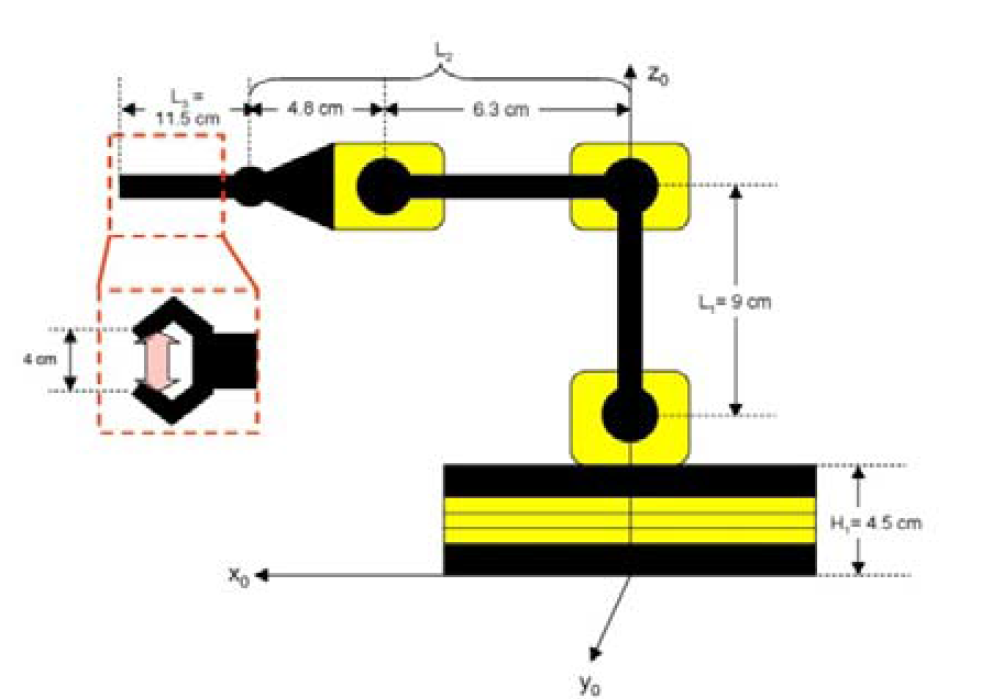
\includegraphics[width=.8\linewidth]{./Images/OWIDIM}
    \caption{Dimensions of the OWI-535 robot arm manipulator\cite{Pradya}}
    \label{fig:OWIDIM}
  \end{minipage}%
\begin{minipage}{.5\textwidth}
\centering
  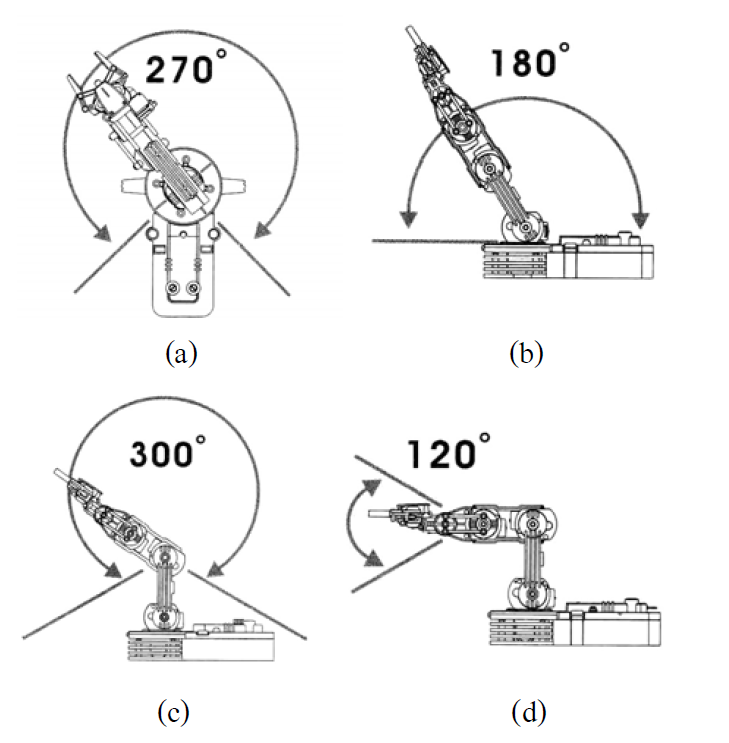
\includegraphics[width=.8\linewidth]{./Images/OWI_LIMITS}
  \caption{Limitation of angular rotation of each joint\cite{Pradya}}
  \label{fig:OWI_LIMITS}
\end{minipage} 
\end{figure}


With the dimensions known, coordinate frames from 0 to 4 are assigned to each link of the robot manipulator. The OWI-535 robot is represented symbolically by figure~\ref{fig:frame_assign} and the frame assignment is also represented on the same figure. The z axis of frame 0 is pointing upward, while the z axes of frame 1 to 4 are parallel and pointing out from the paper. 

\begin{figure}[h!]
  \centering
    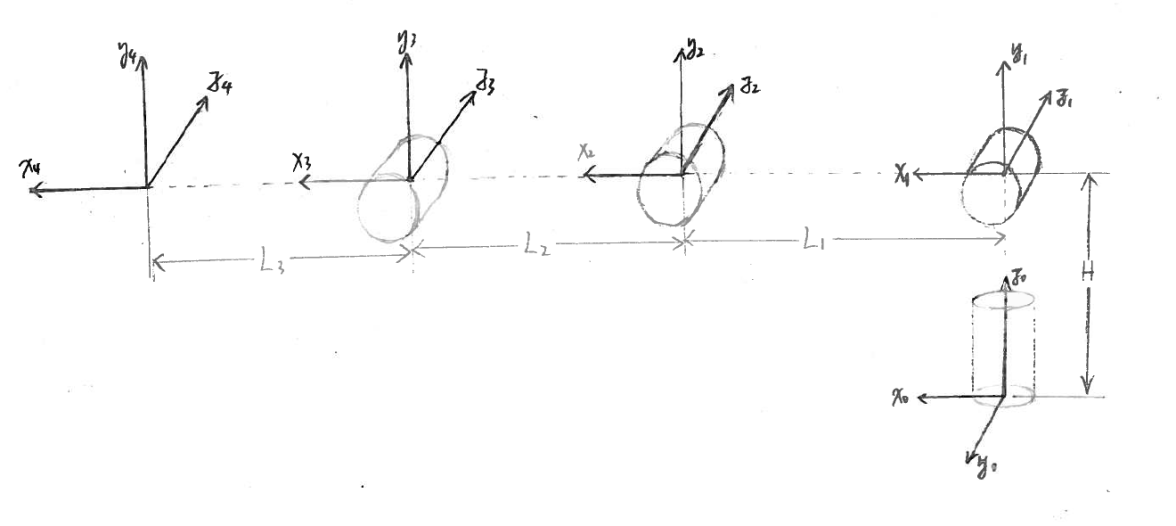
\includegraphics[width=1\textwidth]{./Images/frame_assign}
    \caption{DH coordinate frame assignment for the OWI-535 robot arm manipulator}
    \label{fig:frame_assign}
\end{figure}
Following the Denavit-Hartenberg convention, the DH parameters for each link are shown in table~\ref{tab:DH}, where $H1$, $L1$, $L2$, $L3$ are represented in Figure~\ref{fig:frame_assign}.

\begin{table} 
\caption{DH parameters for OWI-535 robot arm manipulator}
\label{tab:DH}
\begin{center}
\begin{tabular}{lcccc}
\toprule
Link & $a$ & $\alpha$ & $d$ & $\theta$\\
\midrule
1 & 0 & $90^\circ$ & $4.5 cm$ & $\theta_1$\\
2 & $9 cm$ & 0 & 0 & $\theta_2$\\
3 & $11.1 cm$ & 0 & 0 & $\theta_3$\\
4 & $11.5 cm$ & 0 & 0 & $\theta_4$\\
\bottomrule
\end{tabular}
\end{center}
\end{table}

The A matrices for joint 1 to 4 are derived from the table above with equation \eqref{eq:DH}.


%Ai EQUATION
\begin{equation}\label{eq:DH}
{{A}_{i}}=Ro{{t}_{z,{{\theta }_{i}}}}Tran{{s}_{z,{{d}_{i}}}}Tran{{s}_{x,{{a}_{i}}}}Ro{{t}_{x,{{\alpha }_{i}}}}  
\end{equation}

The forward kinematics from frame $0$ to frame $4$ can be then computed by the transform matrix $T_{4}^{0}={{A}_{1}}{{A}_{2}}{{A}_{3}}{{A}_{4}}$, which denote the position and orientation of the end-effector of the robot manipulator. The A matrices and the transform matrix are given in Appendix~\ref{App:AppendixA}.

A MATLAB\textsuperscript{\textregistered} model of the OWI-535 robot arm is generated and the graph of the robot arm at its initial position is presented in the Figure~\ref{fig:OWI_INITIAL_POSITION}.

\begin{figure}[h!]
  \centering
    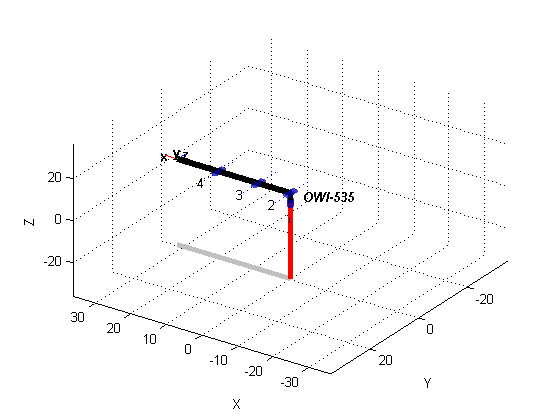
\includegraphics[width=.5\textwidth]{./Images/OWI_INITIAL_POSITION}
    \caption{OWI-535 robot arm at its initial position}
    \label{fig:OWI_INITIAL_POSITION}
\end{figure}
\subsection{Velocity Kinematics and the Jacobian}
At a certain configuration, the velocity relationship between the end-effector and the joint positions are determined by the Jacobian. The Jacobian matrix relates the end-effector linear velocity and angular velocity with the speed of four revolute joints as shown in Equation~\eqref{eq:Jacobian}.

\begin{align} \label{eq:Jacobian}
	\begin{bmatrix} V_x \\
	V_y \\
	V_z \\
	\omega_x \\
	\omega_y \\
	\omega_z
	\end{bmatrix} = 
	\begin{bmatrix}
	\partial x / \partial \theta_1 & \partial x / \partial \theta_2 & \partial x / \partial \theta_3 & \partial x / \partial \theta_4 \\
  	\partial y / \partial \theta_1 & \partial y / \partial \theta_2 & \partial y / \partial \theta_3 & \partial y / \partial \theta_4 \\
  	\partial z / \partial \theta_1 & \partial z / \partial \theta_2 & \partial z / \partial \theta_3 & \partial z / \partial \theta_4 \\
  	\partial \psi / \partial \theta_1 & \partial \psi / \partial \theta_2 & \partial \psi / \partial \theta_3 & \partial \psi / \partial \theta_4 \\
  	\partial \theta / \partial \theta_1 & \partial \theta / \partial \theta_2 & \partial \theta / \partial \theta_3 & \partial \theta / \partial \theta_4 \\
  	\partial \phi / \partial \theta_1 & \partial \phi / \partial \theta_2 & \partial \phi / \partial \theta_3 & \partial \phi / \partial \theta_4
	\end{bmatrix}
	\begin{bmatrix} \dot{\theta_1} \\
	\dot{\theta_2} \\
	\dot{\theta_3} \\
	\dot{\theta_4}
	\end{bmatrix}
\end{align}

For revolute joints, the Jacobian matrix can be determined by the following equations
\begin{align} \label{eq:Jacobian2}
	J = 
	\begin{bmatrix}
	J_{v1} & \cdots  & J_{vn} \\
  	J_{\omega 1} & \cdots & J_{\omega n} \\
	\end{bmatrix} where
\end{align}
\begin{align}
{J_{vi}} = {z_{i - 1}} \times ({o_n} - {o_{i - 1}})\quad & and \quad {J_{\omega i}} = {z_{i - 1}}
\end{align}

This way the Jacobian for a configuration $(\theta_1, \theta_2, \theta_3, \theta_4)$ is determined and the entries of the Jacobian matrix are listed in Appendix~\ref{App:AppendixB}.
\subsection{Simulation}
Using the equations developed in Section~\ref{sec:RMRC}, we simulated moving the robotic arm from:
\[\theta = \begin{matrix}
[0&90^\circ&0&0]
\end{matrix}\]
We set the desired position and speed as
\[x_d = \begin{matrix}
[15&15&3]cm
\end{matrix}\] and
\[\dot{x_d} = \begin{matrix}
[0.2&0.01&0.05]cm/s
\end{matrix}\] respectively.

As can be seen in Figure~\ref{fig:sim}, we see that the arm approaches the desired location at a fixed speed. The code used to complete the simulation can be found in Appendix~\ref{App:AppendixC}.
\begin{figure}[!h]
  \centering
    \includegraphics[width=.75\textwidth]{./Images/sim}
    \caption{OWI-535 robot RMRC Simulation}
    \label{fig:sim}
\end{figure}

\subsection{Workspace Limits}
In order to complete the project, we need to modify our algorithm to stay within the workspace of the robot. After this is complete we will implement the RMRC OWI Robotic ARM.

\subsection{Dynamics}

****** DYNAMICS SECTION *******

\begin{figure}[!h]
  \centering
   \subfloat[Simulation drawing $M$]{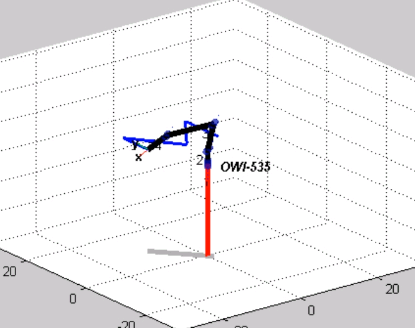
\includegraphics[width=.4\textwidth]{./Images/MPlot}}\quad
   \subfloat[Torques during simulation]{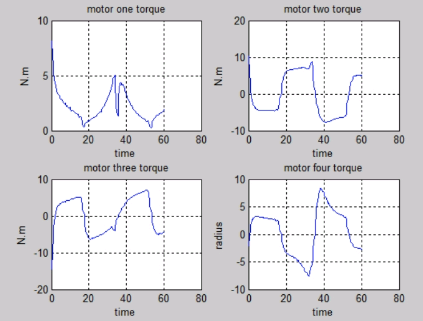
\includegraphics[width=.4\textwidth]{./Images/MTorque}}
    \caption{Dynamic Simulation}
    \label{fig:Simulation}
\end{figure}

\section{Implementation}
This section gives an overview of the implementation of the RMRC on the OWI robot.

\subsection{Hardware Modifications}
The stock OWI robot is controlled by a controller with toggle switches. No method of automatic controller or position feedback is provided. In order to implement the RMRC method, we had to modify the robot with 5 H-Bridge motor controllers and add absolute positional feedback. 
The motor control is completed with a Arduino Uno with a EMGRobotics Six Pack, Figure~\ref{fig:Hardware}. The six pack includes 3 FAN82000 Dual H-Bridges. 

\begin{figure}[!h]
  \centering
   \subfloat[EMG Robtoics Six Pack]{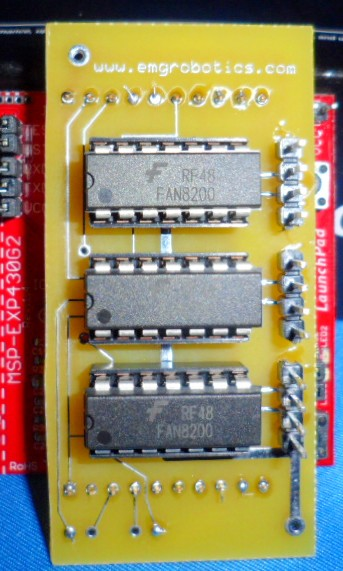
\includegraphics[width=.2\textwidth, angle=90]{./Images/SixPackV1}}\quad
   \subfloat[Arduino Uno]{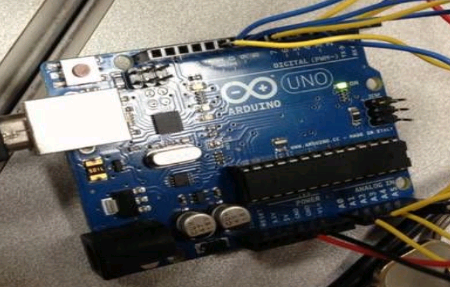
\includegraphics[width=.25\textwidth]{./Images/Uno}}
    \caption{Electronics Hardware}
    \label{fig:Hardware}
\end{figure}

In order to get positional feedback we had to design a way to mount potentiometers to each joint. Each potentiometer is 0-10K$\Omega$, and is used to give the absolute position back to the Arduino. As seen in Figure~\ref{fig:PotMounting}, all potentionmeters are were located on the axis of the joint to allow measuring the full motion of each joint.

\begin{figure}
\centering

\subfloat[Base]{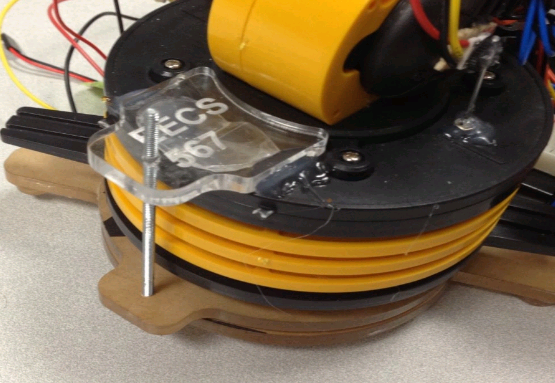
\includegraphics[width=.3\textwidth]{./Images/PotBase}}\quad
\subfloat[Joint 1]{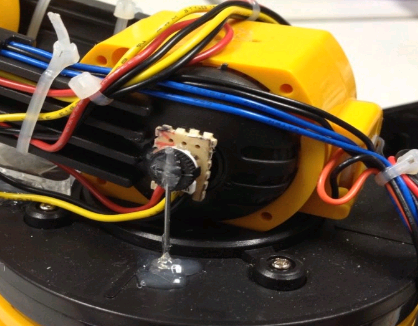
\includegraphics[width=.3\textwidth]{./Images/PotJoint2}}\quad
\subfloat[Joint 2]{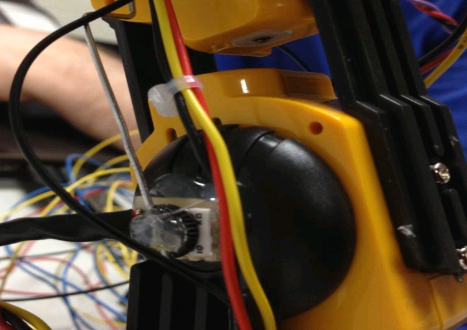
\includegraphics[width=.3\textwidth]{./Images/PotJoint3}}\\
\subfloat[Joint 3]{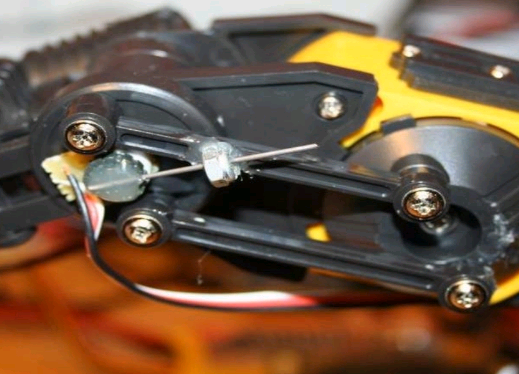
\includegraphics[width=.3\textwidth]{./Images/PotJoint4}}\quad
\subfloat[Joint 4]{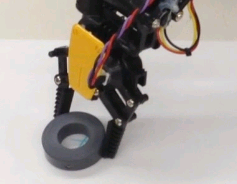
\includegraphics[width=.3\textwidth]{./Images/PotJoint5}}
\caption{Potentiometer Mountings}
\label{fig:PotMounting}
\end{figure}


Currently, the software only allows full on/off control of the motors. To implement the RMRC method we will modify the software to allow Pulse Width Modulation (PWM) control.

\subsection{Software Implementation}

The motor control was implemented using a Proportional Integral (PI) loop on the Arduino. When the Arduino boots up, it captures the current joint positions of each arm and set this postion as the current target. The Arduino then waits for serial commands to set the newest joint location. Each joint can be commanded to a position using a command structure in HEX
\begin{center}
COMMAND = 0x55 0xAA 0x0J 0x\#\#
\end{center}

After receiving the command, the Arduino will move the joint to this location. All joints can operate concurrently and joint positions can be changed rapidly (sub 1 ms).

In MATLAB\textsuperscript{\textregistered}, we setup a serial port class that automatically handles receiving the postional data from the Arduino. The setup of this class is important for recreating the work or similar tasks so it is included in Listing~\ref{lst:setup}.

After Serial communication is established, the user can send commands to Arduino using the function setJointPostion shown in Listing~\ref{lst:setJointPosition}. This function takes the desired joint and angle that matches the DH convention for the robot, formats it, and sends it to the Arduino.
	 
	 \begin{listing}%[H]    
        \caption{Main Loop}    
        \inputminted[linenos=true,frame=lines]{matlab}{src/SerialSetup.m}    
        \label{lst:setup}    
    \end{listing}


	\begin{listing}%[H]
    \caption{Serial Port Setup} 
    \begin{minted}[linenos=true,frame=lines]{matlab}
    
    function setJointPos(Obj,Joint,Position)
%setJointPos Serial object, Joint Num (0-4), Desired Postion(Degrees)
%   Includes bounds checking for angle. 

	\end{minted}
	\label{lst:setJointPosition}1
	\end{listing}

Using the functions created above, we created a program in MATLAB\textsuperscript{\textregistered} that runs our RMRC algorithm and sends the positions to the Arduino. It sends the first four joint locations, can constantly calculates the max error of all joints. When the max error falls below a given threshold, the program sends the next command sequence. 
	
\section{Testing}

After building the hardware and completing the software, our team ran tests using the modified OWI robot. We set out to complete two objectives. The first was to complete a task, by defining the the way points at each several positions and having the robot move through each. The task was setup to have the robot move a washer from one location to another similar to a pick and place machine. This task was selected as it allowed us to understand the control algorithm tuning and verify the robot was ready to test RMRC. Figure~\ref{fig:task} shows the robot picking up the washer.

The second objective was to test the RMRC algorithm on the robot. We decided to have the robot paint a line on a piece of paper. This task was completed by setting up a line in the work space using MATLAB\textsuperscript{\textregistered} and specifying the desired speed in World Coordinates. Figure~\ref{fig:Testing} shows the robot painting a line. 


\begin{figure}[!h]
  \centering
   \subfloat[\label{fig:task} Completing Task]{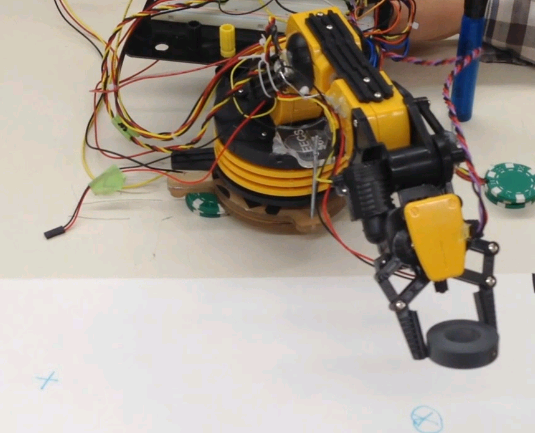
\includegraphics[width=.4\textwidth]{./Images/Task}}\quad
   \subfloat[\label{fig:path}Following Path]{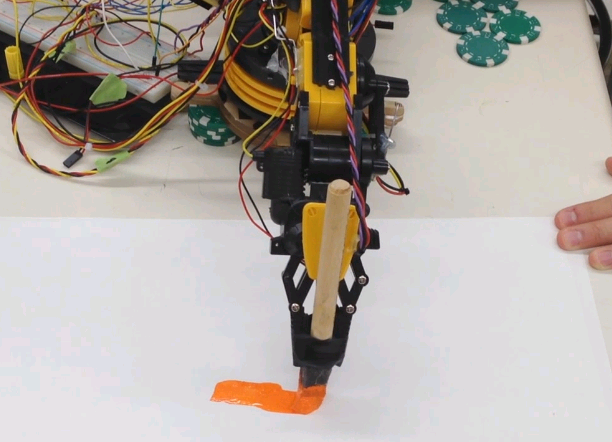
\includegraphics[width=.4\textwidth]{./Images/DrawLine}}
    \caption{Physical Testing}
    \label{fig:Testing}
\end{figure}

\subsection{Challenges}
The testing showed the limitations of the hardware we were using. Although the simulation operated smoothly, the robot movement was jerky with limited resolution of the encoder and low power motors operating high friction joints.

In future implementations it is recommended to use high resolution encoders so speed control is possible and investigate higher power motor with lower gear lash. As well, once speed control is available, it is recommended that the full algorithm be implemented on a microprocessor to allow stand alone operation using a fixed point math. 

\section{Conclusion}

Overall, the RMRC method allows for simple iterative method to follow a path. The advantage is that it could be used in real time on a controller using lookup tables for sin and cosine and pointer matrix math. Ideal situations would be on mobile robots that include manipulators that are human controlled live.

Our implementation was not in real time but did add both joint limitation considerations and investigated dynamics beyond the standard RMRC algorithms we studied. 

\bibliographystyle{IEEEtran}
\bibliography{EECS567_Refs}
\newpage
\appendix
\section{\\Denavit-Hartenberg Matrices} \label{App:AppendixA}
\begin{align} 
	A_1 = 
	\begin{bmatrix}
	\cos_1 	& 0  & \sin_1 	& 0 \\
  	\sin_1 	& 0  & -\cos_1 	& 0 \\
  	0		& 1  & 0 		& H \\
  	0		& 0  & 0 		& 1 
	\end{bmatrix} &&
	A_2 = 
	\begin{bmatrix}
	\cos_2 	& -\sin_2  & 0 	& L_1\cos_2 \\
  	\sin_2 	& \cos_1  & 0 	& L_1\sin_2 \\
  	0		& 0  & 1 		& 0 \\
  	0		& 0  & 0 		& 1 
	\end{bmatrix}\\
	A_3 = 
	\begin{bmatrix}
	\cos_3 	& -\sin_3  & 0 	& L_2\cos_3 \\
  	\sin_3 	& \cos_3  & 0 	& L_2\sin_3 \\
  	0		& 0  & 1 		& 0 \\
  	0		& 0  & 0 		& 1 
	\end{bmatrix} && 
	A_4 = 
	\begin{bmatrix}
	\cos_4 	& -\sin_4  & 0 	& L_3\cos_4 \\
  	\sin_4 	& \cos_4  & 0 	& L_3\sin_4 \\
  	0		& 0  & 1 		& 0 \\
  	0		& 0  & 0 		& 1 
	\end{bmatrix}
\end{align}

\begin{align}
T_4^0 = 
	\begin{bmatrix}
	\cos_1 \cos_{234} 	& -\cos_1 \sin_{234} 	& \sin_1 	& (L_1\cos_2+L_2\cos_{23}+L_3\cos_{234})\cos_1 \\
  	\sin_1 \cos_{234} 	& -\sin_1 \sin_{234}  	& -\cos_1 	& (L_1\cos_2+L_2\cos_{23}+L_3\cos_{234})\sin_1 \\
  	\sin_{234}			& \cos_{234}  			& 0 		& L_1\cos_2+L_2\cos_{23}+L_3\cos_{234} + H \\
  	0					& 0  					& 0 		& 1 
	\end{bmatrix}
\end{align}


\newpage
\section{\\Jacobian Matrix Entries} \label{App:AppendixB}


\[\partial x/\partial {\theta _1} =  - ({L_1}{C_2} + {L_2}{C_{23}} + {L_3}{C_{234}}){S_1}\]
\[\partial x/\partial {\theta _2} =  - ({L_1}{S_2} + {L_2}{S_{23}} + {L_3}{S_{234}}){C_1}\]
\[\partial x/\partial {\theta _3} =  - ({L_2}{S_{23}} + {L_3}{S_{234}}){C_1}\]
\[\partial x/\partial {\theta _4} =  - ({L_2}{S_{23}} + {L_3}{S_{234}}){C_1}\]
\[\partial y/\partial {\theta _1} = ({L_1}{C_2} + {L_2}{C_{23}} + {L_3}{C_{234}}){C_1}\]
\[\partial y/\partial {\theta _2} =  - ({L_1}{S_2} + {L_2}{S_{23}} + {L_3}{S_{234}}){S_1}\]
\[\partial y/\partial {\theta _3} =  - ({L_2}{S_{23}} + {L_3}{S_{234}}){S_1}\]
\[\partial y/\partial {\theta _4} =  - ({L_3}{S_{234}}){S_1}\]
\[\partial z/\partial {\theta _1} = 0\]
\[\partial z/\partial {\theta _2} = ({L_1}{C_2} + {L_2}{C_{23}} + {L_3}{C_{234}})\]
\[\partial z/\partial {\theta _3} = ({L_2}{C_{23}} + {L_3}{C_{234}})\]
\[\partial z/\partial {\theta _3} = {L_3}{C_{234}}\]
\[\partial \psi /\partial {\theta _1} = 0\]
\begin{center}
$\partial \psi /\partial {\theta _i} = {S_1}	\text{ where i}=2,3,4$
\end{center}

\[\partial \theta /\partial {\theta _1} = 0\]
\begin{center}
$\partial \theta /\partial {\theta _i} =  - {C_1}	\text{ where i}=2,3,4$
\end{center}

\[\partial \phi /\partial {\theta _1} = 1\]
\begin{center}
$\partial \phi /\partial {\theta _i} = 0		\text{ where i}=2,3,4$
\end{center}
\newpage

\section{\\Source Code} \label{App:AppendixC}

The code for this project was created using Arduino IDE V1.1 and MATLAB\textsuperscript{\textregistered} R2011b. The project utilizes open source Arduino Libraries and the code has been setup for future use.

The MATLAB\textsuperscript{\textregistered} files included customizable functions for receiving Serial Data and sending Serial Data via RS-232 with the Arudino Uno or other similar RS-232 device.

All source code and MATLAB\textsuperscript{\textregistered} files can be found on GitHub repository at

\begin{center}
\textbf{https://github.com/kjschill/OWI\_ARM}
\end{center}

As well, the project files have been uploaded to CTools site for EECS567 W13 class projects.

For access to the project, please contact:
\begin{center}
Kris Schilling
\\kjschill@umich.edu
\\University of Michigan
\end{center}

\end{document}

